\section{\texorpdfstring{ADC - analogově digitální převod}{ADC - analogove digitalni prevod}}

% =====================================================================================================================
	\begin{frame}
    \frametitle{ADC}

		\textbf{Základní parametry}
		
		\begin{itemize}
			\item Přesnost převodu je 10 bit, výsledek $\in \left\langle 0, 1024 \right\rangle$,
			\item pro tuto funkci je vyhrazeno 10 pinů: \textbf{PB0} až \textbf{PB7}, \textbf{PE6} a \textbf{PE7},
			\item převodní jednotka je jen jedna $\Rightarrow$ mezi piny se provádí multiplex,
			\item převod se provádí pomocí postupné aproximace $\Rightarrow$ 14 cyklů,
			\item vektor přerušení pro konec převodu (získání výsledku).
		\end{itemize}
		
		\begin{center}
			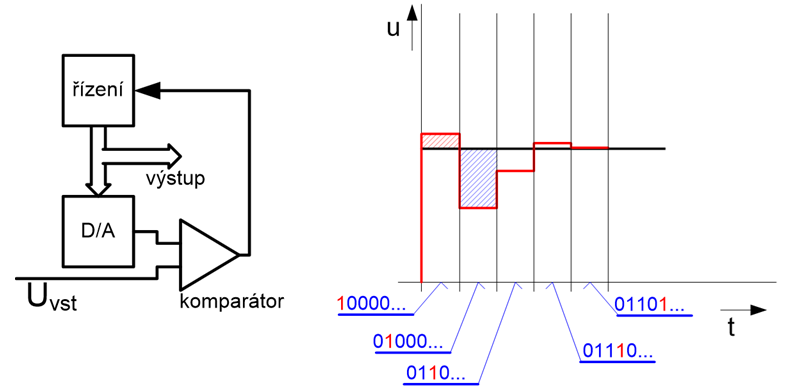
\includegraphics[width=0.7\textwidth]{fig/adc_succesive_approx.png}
		\end{center}
		
	\end{frame}

% =====================================================================================================================
	\begin{frame}
    \frametitle{Návod v materiálech na cvičení}

		\begin{center}
			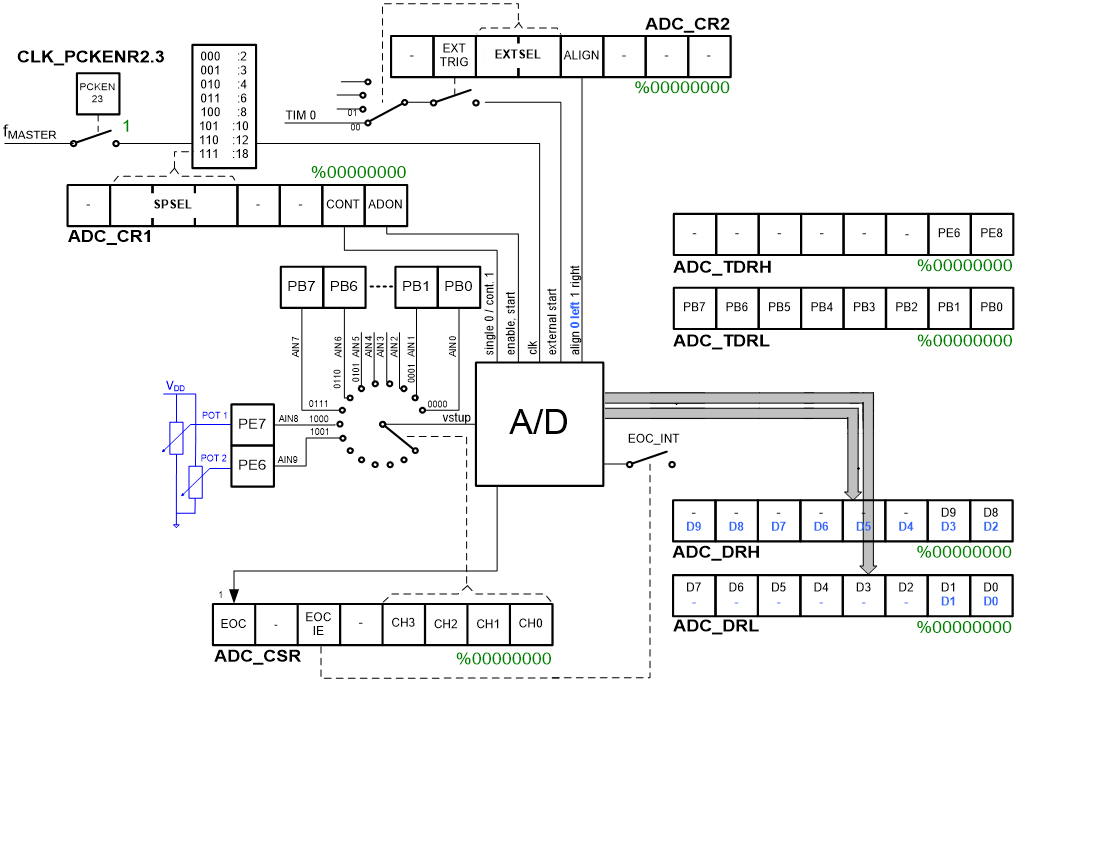
\includegraphics[width=1.00\textwidth]{fig/adc_navod.png}
		\end{center}
		
	\end{frame}
	
% =====================================================================================================================
	\begin{frame}
    \frametitle{Význam registru ADC\_CSR}

		\textbf{C}ontrol/\textbf{S}tatus \textbf{R}egister

\begin{center}
			\tiny
			\begin{tabular}{| p{9mm} | p{9mm} | p{9mm} | p{9mm} | p{9mm} | p{9mm} | p{9mm} | p{9mm} |}
				\hline
				\hline
				\textbf{EOC} & \textcolor{red}{\textbf{AWD}} & \textbf{EOCIE} & \textcolor{red}{\textbf{AWDIE}} & \textbf{CH3} & \textbf{CH2} & \textbf{CH0} & \textbf{CH0} \\
				\hline
				\hline
			\end{tabular}
		\end{center}
				
		\begin{itemize}
			\item slouží pro volbu vstupu, kde bude získáván vzorek měření a k signalizaci konce převodu,
			\item stav po resetu 0x00,
			\small
			\begin{center}
				\begin{tabular}{l p{80mm}}
					\textbf{EOC} & Konec převodu vystaví tento bit do 1 (pokud byl v 0). \\
					\textcolor{red}{\textbf{AWD}} & Povolení pro analogový watchdog, hlídá stanovené úrovně, \textbf{toto neřešíme}. \\
					\textbf{EOCIE} & Povolení přerušení na konci převodu. \\
					\textcolor{red}{\textbf{AWDIE}} & Povolení přerušení pro watchdog, \textbf{toto neřešíme}. \\
					\textbf{CH3:0} & Adresa pinu pro převod.
				\end{tabular}
			\end{center}
		\end{itemize}
		
	\end{frame}

% =====================================================================================================================
	\begin{frame}
    \frametitle{Adresa pinu - multiplexer}
		
		
		\begin{center}
			\begin{tabular}{c | c || c | c}
				\textbf{CH3:0} & Pin převodu & \textbf{CH3:0} & Pin převodu \\
				\hline
				0000 & \textbf{PB0} & 0101 & \textbf{PB5} \\
				0001 & \textbf{PB1} & 0110 & \textbf{PB6} \\
				0010 & \textbf{PB2} & 0111 & \textbf{PB7} \\
				0011 & \textbf{PB3} & 1000 & \textcolor{blue}{\textbf{PE7}} \\
				0100 & \textbf{PB4} & 1001 & \textcolor{blue}{\textbf{PE6}} \\
			\end{tabular}
		\end{center}
		
		\vspace{5mm}
		Na přípravku lze použít piny PE7 a PE6, kam jsou přivedeny signály z jezdců potenciometrů.
		
	\end{frame}
	
% =====================================================================================================================
	\begin{frame}
    \frametitle{Význam registru ADC\_CR1}

		\textbf{C}ontrol \textbf{R}egister 1

\begin{center}
			\tiny
			\begin{tabular}{| p{9mm} | p{9mm} | p{9mm} | p{9mm} | p{9mm} | p{9mm} | p{9mm} | p{9mm} |}
				\hline
				\hline
				\textbf{-} & \textbf{SPSEL2} & \textbf{SPSEL1} & \textbf{SPSEL0} & \textbf{-} & \textbf{-} & \textbf{CONT} & \textbf{ADON} \\
				\hline
				\hline
			\end{tabular}
		\end{center}
				
		\begin{itemize}
			\item slouží pro nastavení předděličky hodin a pro nastavení spuštění ADC,
			\item stav po resetu 0x00,
			\small
			\begin{center}
				\begin{tabular}{l p{80mm}}
					\textbf{SPSEL2:0} & Předdělička hodin - úspora energie \\
					\textbf{CONT} & Režim spouštění AD převodu, \textbf{0}: na povel, \textbf{1}: vždy \\
					\textbf{ADON} & Povolení přerušení na konci převodu. \\
				\end{tabular}
			\end{center}
		\end{itemize}
		
		\begin{center}
		\small
			\begin{tabular}{c | c || c | c}
				\textbf{SPSEL2:0} & Pin převodu & \textbf{SPSEL2:0} & Pin převodu \\
				\hline
				000 & $f_{M}/2$ & 100 & $f_{M}/8$ \\
				001 & $f_{M}/3$ & 101 & $f_{M}/10$ \\
				010 & $f_{M}/4$ & 110 & $f_{M}/12$ \\
				011 & $f_{M}/6$ & 111 & $f_{M}/18$ \\
			\end{tabular}
		\end{center}
	\end{frame}
	
% =====================================================================================================================
	\begin{frame}
    \frametitle{Význam registru ADC\_CR2}

		\textbf{C}ontrol \textbf{R}egister 2

\begin{center}
			\tiny
			\begin{tabular}{| p{9mm} | p{9mm} | p{9mm} | p{9mm} | p{9mm} | p{9mm} | p{9mm} | p{9mm} |}
				\hline
				\hline
				\textbf{-} & \textcolor{red}{\textbf{EXTRIG}} & \textcolor{red}{\textbf{EXTSEL1}} & \textcolor{red}{\textbf{EXTSEL0}} & \textbf{ALIGN} & \textbf{-} & \textcolor{red}{\textbf{SCAN}} & \textbf{-} \\
				\hline
				\hline
			\end{tabular}
		\end{center}
				
		\begin{itemize}
			\item slouží pro nastavení externího spouštění a zarovnání výsledku,
			\item stav po resetu 0x00,
			\small
			\begin{center}
				\begin{tabular}{l p{80mm}}
					\textcolor{red}{\textbf{EXTRIG}} & Povolení externího spouštění, \textbf{toto neřešíme}. \\
					\textcolor{red}{\textbf{EXTSEL1:0}} & Výběr zdroje externího spouštění, \textbf{toto neřešíme}. \\
					\textbf{ALIGN} & Zarovnání výsledku do 16 bitů. \\
					\textcolor{red}{\textbf{SCAN}} & Scan mode, všechny analogové vstupy se postupně převádějí, HW sám mění adresu pinu, \textbf{toto neřešíme}. \\
				\end{tabular}
			\end{center}
		\end{itemize}
	\end{frame}
	
% =====================================================================================================================
	\begin{frame}
    \frametitle{Zarovnání výsledku v registrech ADC\_DRH a ADC\_DRL}
		
		\begin{itemize}
			\item Registry zaznamenávají výsledek převodu,
			\item hodnotu zadává HW.
		\end{itemize}
		
		\vspace{3mm}
		\textbf{ALIGN = 0}, zarovnání vlevo
		
		\begin{center}
		\textbf{ADC\_DRH:}
			\begin{tabular}{ | p{5mm} | p{5mm} | p{5mm} | p{5mm} | p{5mm} | p{5mm} | p{5mm} | p{5mm} |}
				\hline
				\hline
				\textbf{b9} & \textbf{b8} & \textbf{b7} & \textbf{b6} & \textbf{b5} & \textbf{b4} & \textbf{b3} & \textbf{b2} \\
				\hline
				\hline
			\end{tabular}
		\end{center}
		
		\begin{center}
		\textbf{ADC\_DRL:}
			\begin{tabular}{ | p{5mm} | p{5mm} | p{5mm} | p{5mm} | p{5mm} | p{5mm} | p{5mm} | p{5mm} |}
				\hline
				\hline
				\textbf{0} & \textbf{0} & \textbf{0} & \textbf{0} & \textbf{0} & \textbf{0} & \textbf{b1} & \textbf{b0} \\
				\hline
				\hline
			\end{tabular}
		\end{center}
		
		\vspace{3mm}
		\textbf{ALIGN = 1}, zarovnání vpravo
		
		\begin{center}
		\textbf{ADC\_DRH:}
			\begin{tabular}{ | p{5mm} | p{5mm} | p{5mm} | p{5mm} | p{5mm} | p{5mm} | p{5mm} | p{5mm} |}
				\hline
				\hline
				\textbf{0} & \textbf{0} & \textbf{0} & \textbf{0} & \textbf{0} & \textbf{0} & \textbf{b9} & \textbf{b8} \\
				\hline
				\hline
			\end{tabular}
		\end{center}
		
		\begin{center}
		\textbf{ADC\_DRL:}
			\begin{tabular}{ | p{5mm} | p{5mm} | p{5mm} | p{5mm} | p{5mm} | p{5mm} | p{5mm} | p{5mm} |}
				\hline
				\hline
				\textbf{b7} & \textbf{b6} & \textbf{b5} & \textbf{b4} & \textbf{b3} & \textbf{b2} & \textbf{b1} & \textbf{b0} \\
				\hline
				\hline
			\end{tabular}
		\end{center}

	\end{frame}
	
% =====================================================================================================================
	\begin{frame}
    \frametitle{Registry ADC\_TDRH a ADC\_TDRL - nastavení pinu}
		
		\begin{center}
			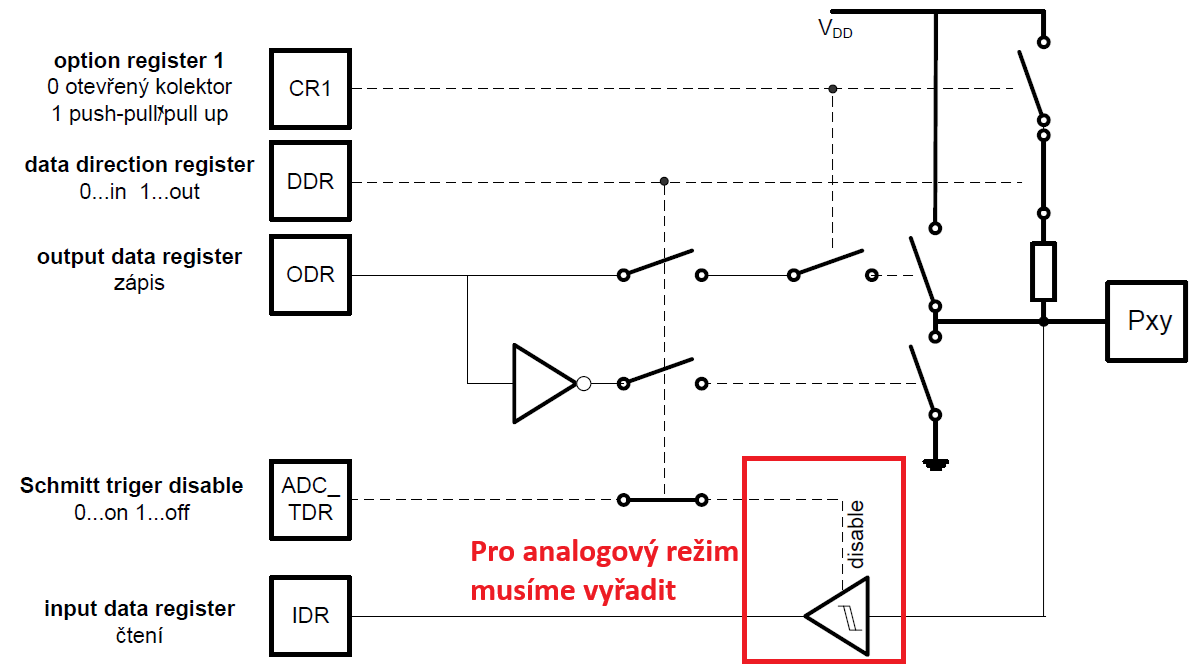
\includegraphics[width=0.80\textwidth]{fig/pin_settings_adc.png}
		\end{center}

	\end{frame}
	
% =====================================================================================================================
	\begin{frame}
    \frametitle{Registry ADC\_TDRH a ADC\_TDRL}
		
		\begin{itemize}
			\item slouží k vyřazení shmittova klopného obvodu,
			\item příslušný bit odpovídá číslu kanálu \textbf{AIN = CH3:0}, viz registr \textbf{ADC\_CSR},
			\item pro vyřazení zapisujeme na příslušný bit 1.
		\end{itemize}
		
		\vspace{3mm}
		
		\begin{center}
		\textbf{ADC\_TDRH:}
			\begin{tabular}{ | p{7mm} | p{7mm} | p{7mm} | p{7mm} | p{7mm} | p{7mm} | p{7mm} | p{7mm} |}
				\hline
				\hline
				\textbf{0} & \textbf{0} & \textbf{0} & \textbf{0} & \textbf{0} & \textbf{0} & \textbf{PE6} & \textbf{PE7} \\
				\hline
				\hline
			\end{tabular}
		\end{center}
		
		\begin{center}
		\textbf{ADC\_TDRL:}
			\begin{tabular}{ | p{7mm} | p{7mm} | p{7mm} | p{7mm} | p{7mm} | p{7mm} | p{7mm} | p{7mm} |}
				\hline
				\hline
				\textbf{PB7} & \textbf{PB6} & \textbf{PB5} & \textbf{PB4} & \textbf{PB3} & \textbf{PB2} & \textbf{PB1} & \textbf{PB0} \\
				\hline
				\hline
			\end{tabular}
		\end{center}

	\end{frame}
	
% =====================================================================================================================
	\begin{frame}
    \frametitle{Program vyčtení ADC }
		
		\begin{enumerate}
			\item Nastavit periferii ADC pro jednotlivá čtení vstupu PE6,
			\item spustit převod a vyčkat dokončení,
			\item výsledek zobrazit na výstupních LED,
			\item vyčkat pomocí funkce \uv{wait}.
			\item opakovat postup od bodu 2.
		\end{enumerate}
		
	\end{frame}
	
% =====================================================================================================================
	\begin{frame}
    \frametitle{Program vyčtení ADC - zdrojový kód}
		
		\begin{center}
			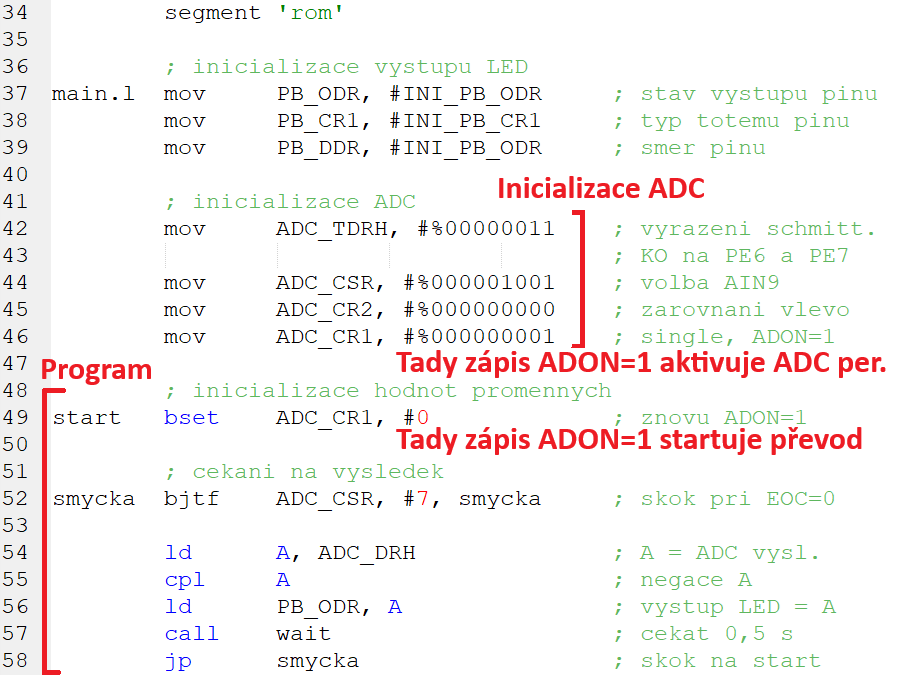
\includegraphics[width=0.80\textwidth]{fig/prg_adc.png}
		\end{center}
		
	\end{frame}